%----Preamble-------------------------------------------------------------
\documentclass[	a4paper,
				11pt,
				DIV=11,
				bigheadings,
				idxtotoc,
				listof=totoc,	
				bibtotoc,		
				halfparskip,
				cleardoubleempty,
				oneside,
				openright]{scrartcl}

%--------Packages--------------------------------------------------------------------------

\usepackage[english]{babel}
\usepackage[T1]{fontenc} 	
\usepackage[utf8]{inputenc}
\usepackage{enumitem}
\usepackage{graphicx}	
\usepackage[labelfont=bf]{caption}
\usepackage{float}
\usepackage{wrapfig}
\usepackage{geometry}
\geometry{a4paper,left=30mm,right=20mm}
\usepackage{blindtext}
\usepackage{layout}
\PassOptionsToPackage{hyphens}{url}		
\usepackage[pdfborder={0 0 0},
			colorlinks=true, 
			linkcolor=black,
			citecolor=blue,
			]{hyperref}
\usepackage[backend=bibtex,style=numeric,sorting=none]{biblatex}
\addbibresource{literature.bib}
\usepackage{pdfpages}
\usepackage{color}
\usepackage{xcolor}
\usepackage{setspace}
\usepackage[toc,page]{appendix}
\usepackage{longtable}
\usepackage{multirow}
\usepackage{colortbl}
\usepackage{parskip}
\usepackage{enumitem}
\usepackage{makecell}
\renewcommand\theadfont{\bfseries\sffamily}
\usepackage{amsmath}
\usepackage{amssymb}
\DeclareMathOperator{\E}{E}
\usepackage{scrlayer-scrpage}
\pagestyle{scrheadings}							
\clearscrheadfoot 						
\ohead{\pagemark}								
\ihead{\ifthispageodd{\leftmark}{\rightmark}} 	
\setheadsepline{0.4pt} 							
\setkomafont{pagehead}{\scshape}		
\setfootsepline{0.4pt} 							
\setkomafont{pagefoot}{\scshape}				
\ifoot{\footnotesize{Daniil Navodey}}
\ofoot{\footnotesize{THI Ingolstadt}}		


\defpagestyle{myPageStyle}{
	(0pt ,0pt)
	{\hfill\pagemark} {\hfill\pagemark} {\hfill\pagemark}
	(0pt ,0pt)	
}{
{
	(\textwidth ,0.4pt)
	\footnotesize{Daniil Navodey} \hfill \footnotesize{THI Ingolstadt}} 
	{\footnotesize{Daniil Navodey} \hfill \footnotesize{THI Ingolstadt}} 
	{\footnotesize{Daniil Navodey} \hfill \footnotesize{THI Ingolstadt}}
	(0pt ,0pt)
}


%----Colour definition------------------------------------------------------
\definecolor{haw_mag}{rgb}{0,0.112,0.47}
\addtokomafont{section}{\color{haw_mag} \rmfamily \scshape} 
\addtokomafont{subsection}{\color{haw_mag} \rmfamily}
\addtokomafont{subsubsection}{\color{haw_mag} \rmfamily}
\addtokomafont{paragraph}{\color{haw_mag} \rmfamily}
\addtokomafont{subparagraph}{\rmfamily}

\definecolor{tab_2}{RGB}{230,230,230}
\definecolor{tab_1}{RGB}{85,128,214}

%------Length adjustment--------------------------------------------------------
\setlength{\headsep}{10mm}						
\setlength{\footskip}{15mm}						
\setlength{\textheight}{235mm}					


%----Glossary-------------------------------------------------------------------
\usepackage[toc, acronym]{glossaries} 			
\makeglossaries	

%---Nomenclature----------------------------------------------------------------
\usepackage[intoc]{nomencl} 
\makenomenclature


\includeonly{	
	titlepage,							
	affidavit,
	acknowledgments,
	abstractEN,
	confidentialityClause,
	glossary,
	mainpart,
	nomenclature,
	appendices
	}
	
		
%----------------Beginning of Document---------------------------------------


\begin{document}
	\widowpenalty=10000
	\clubpenalty=10000
	\displaywidowpenalty=10000	
	

	% Title page	
	%----------Title page-------------------------------------------------------------

\newgeometry{textheight=0.9\paperheight, textwidth=0.76\paperwidth, left=30mm, right=20mm}

\begin{titlepage}	
	%----THI-logo--------------------------------------------------------
		\begin{figure}[!h]
			\centering
			
\includegraphics[width={0.5\textwidth}]{images/thiRGB.jpg}	
		\end{figure}																			
	%------------------------------------------------------------------------------
	
	\begin{center}
		\hrulefill 
	\end{center}
	
	
	\begin{center}	
		\vspace{1cm}
		
		\huge\textbf{
			Bachelor Thesis}\\[1em]
		\normalsize
			in the study program \\ B. Eng. in Autonomous Vehicle Engineering\\ Faculty of Electrical Engineering and Information Technology\\ [8em]
	
		\Large\textbf{Leveraging Criticality in Reinforcement Learning for Effective Transfer Learning in Autonomous Driving}	 \\ [10em]

	\end{center}
	
	
	\begin{tabular}{lll}
		First, Last name &:& \textbf{Daniil Navodey}	\\ [1em]
		
		Matriculation number &:& 00126504 \\[3em]
		
		First Examiner &:& Prof. Dr. Lenz Belzner	\\ [1em]
		Second Examiner &:& "Your second examiner here"	\\ [2em]
		
		External guide &:& "Your external guide here" \\[3em]
		
		Institute &:& THI Ingolstadt \\
	\end{tabular}
	
\end{titlepage}

\restoregeometry					
	\cleardoublepage					
	\pagenumbering{Roman} 			
    
    % Affidavit
	\thispagestyle{myPageStyle}
	%----------Affidavit--------------------------------------

\addsec{Affidavit}
I declare that I have authored the present thesis independently and that I have not used any other sources/resources than the ones declared here. I have explicitly indicated all the material which has been quoted either literally or by consent from the sources used and I have marked verbatim and indirect quotations as such. I also declare that I have not presented the work elsewhere for examination purpose.

\vspace*{2.5cm}
	
Ingolstadt, \rule{0.3\textwidth}{0.4pt}	

	
% Signature
Faruk Kahraman

	\cleardoublepage
	
	% Acknowledgements
	\thispagestyle{myPageStyle}
	%----------Acknowledgments--------------------------------------------------------------
\addsec{Acknowledgments}

"Your acknowledgements here."

\vspace*{1.5cm}
		
Daniil Navodey\\
Ingolstadt, Germany

	\cleardoublepage
	
	% Abstract English
	\thispagestyle{myPageStyle}
	%----------Abstract-----------------------------------------------------------
\addsec{Abstract}

While Reinforcement Learning is showing extensive potential in applications which include autonomous driving, its major drawback is the gigantic computing resources and time necessary to train a model from scratch. As a solution, transfer learning was introduced, reducing required data and time when adapting pre-trained models to new environments. However, huge sets of randomly sampled data are traditionally used in transfer learning, introducing great inefficiencies. This research proposes an approach to optimise the standard transfer learning process by leveraging criticality--a measure of the significance of one/more actions in a given state. The training time is reduced when the replay buffer of a model is fed with only critical states during the retraining process while the achieved model performance is maintained comparable to conventional transfer learning. The approach was validated by applying Deep Q-Network (DQN) in \emph{Highway-Env} and \emph{Merge-Env} environments for simulated autonomous driving. Results demonstrate that safety and other performance metrics are evaluated to be comparable for transfer learning based on criticality, although requiring only a fraction of training data. This suggests criticality approach is more feasible for applications in the real world. Insights gathered throughout the thesis will endow the research in the optimisation of machine learning and the development of autonomous driving.
	\cleardoublepage
	
	% Confidentiality clause (from BMW if any)
	\thispagestyle{myPageStyle}
	%----------Confidentiality clause---------------------------------------------------


\addsec{Confidentiality clause}

"Talk to BMW"\\ 
	
Ingolstadt, \rule{0.3\textwidth}{0.4pt}	\\
\textcolor{white}{.}\qquad\qquad\qquad\qquad\quad \small (Date) \\ [1.3cm]
	
(Signature) \\
Daniil Navodey

	\cleardoublepage
	
	% Nomenclature
	\addsec{Nomenclature}

\nomenclature{$\sigma$}{Sigmoid function}
\nomenclature{$w$}{Neural network weights}
\nomenclature{$e$}{Euler's number}
		
	\printnomenclature
	\cleardoublepage	
	
	% Glossary
	%----------Glossary-------------------------------------------------------------

\newglossaryentry{abs}{name={abs},description={Absolute operation}}  

\newacronym{d}{D}{Dimensions}
\newacronym{hsv}{HSV}{Hue Saturation Value channels}
	
	\printglossaries	
	\glsaddallunused
	\cleardoublepage

	
	% List of figures
	\thispagestyle{myPageStyle}
	\renewcommand*\listfigurename{List of figures} 
	\listoffigures
	\cleardoublepage
	
	% List of tables
	\thispagestyle{myPageStyle}
	\renewcommand*\listtablename{List of tables} 
	\listoftables
	\cleardoublepage
	
	% Table of contents
	\thispagestyle{myPageStyle}
	\renewcommand{\contentsname}{Table of contents} 
	\tableofcontents
	\cleardoublepage
	\singlespacing
	
	% Main part of the thesis
	\pagenumbering{arabic} 						
	%----------Main part of the thesis---------------------------------------------------------
\thispagestyle{myPageStyle}
% Chapter 1:
% ----------
\section{Introduction}\label{chap:chap_1}


% Section 1:
%-----------
\subsection{Motivation}
Transportation nowadays has acquired a new round of development with the introduction of autonomous driving technologies based on machine learning (ML), neural networks (NN), and artificial intelligence (AI). This changed how we think about safety, efficiency and accessibility of transport. The key challenge of a self-driving vehicle is the number of decisions, required for an algorithm to be taken in real-time which will cause endangering consequences for drivers, passengers and other traffic participants. Reinforcement Learning (RL) is a promising approach to tackle this challenge because it allows systems to learn by trying different actions and improving over time. However, to train RL sufficiently for real-world driving it needs a lot of time and big data sets for the learning process.\\
The major drawback of RL is the lack of adaptivity of models to new situations. This requires an additional learning process, which is time-consuming and inefficient. This is where Transfer Learning (TL) can help. TL enables the ability of a system to take what it has learned in one situation and then apply gathered knowledge to a new one, with less effort and time taken. Emphasizing the focus of TL to be trained on critical states of the system - the moments where making the right decision matters for safety and performance -  can lead to an exclusive ability to learn faster and perform better under real-world conditions.\\
This thesis explores the approach to make RL better at knowledge transfer in the field of autonomous driving by applying critical situations to the models' training process. The aim is to improve the performance of models, broadening the variety of challenges that could be handled, and ensuring the effectiveness of learning. By addressing these issues, this research could contribute to the further development of autonomous driving systems by making them more practical and reliable.\\


% Section 2:
%-----------
\subsection{Objective}




% Section 3:
%-----------
\subsection{Scope}



% Section 4:
%-----------
\subsection{Commonly used terms}

\begin{enumerate}
	\item \textbf{Commonly used term 1}
	
	\item \textbf{Commonly used term 2}
	
	\item \textbf{Commonly used term 3}
\end{enumerate}


% Section 5:
%-----------
\subsection{Thesis-outline}

\begin{enumerate}[label=\Roman*]
	\item {\color{red} \textbf{Chapter \ref{chap:chap_1}}}: Introduction\\
	
	\item {\color{red} \textbf{Chapter \ref{chap:chap_2}}}: Literature Survey\\
	
	\item {\color{red} \textbf{Chapter \ref{chap:chap_3}}}: Method\\
	 
	\item {\color{red} \textbf{Chapter \ref{chap:chap_4}}}: Experiments, Results and Discussion\\
	
	\item {\color{red} \textbf{Chapter \ref{chap:chap_5}}}: Conclusion\\
    
\end{enumerate}

\newpage

\thispagestyle{myPageStyle}
% Chapter 2:
\section{Literature survey}\label{chap:chap_2}

%-----------
% Section 1: Brief introduction to autonomous driving and it's modules
\subsection{Criticality}\label{sec:subsec_2.1}

One small branch that can be applied to any type of learning which is not explored deep enough and not widely applied yet is criticality. The criticality has varios ways to be computed when used in reinforcement learning and autonomous driving. Despite that the definition of criticality is general for all the possible implementation fields: the higher vallue of criticality corresponce to the lower value of safety and higher threat level\cite{CriticalityAutonomous2023} in a chosen situation. 

In a field of autonomous driving the knowledge of criticality, especially the ability of the machine to approximate this value, is crusial for the algorithms that are either already used or are still under development. The ability of models that control driving behavior to process the environment, observations and disturbances to evaluate the measure for the threat level of the situation in a real-time can boost the performance and increase the reliability of autonomous driving technologies. 

The policy can be a base to calculate necessary value. The criticality of a state can be accessed throught the comparison of an entropy of the policy's output action distribution captured at a state \texttt{s} with the threshold value. In this method the threshold value \texttt{t} is the one controlling the number of states to be considered "critical"~\cite{huang2018establishingappropriatetrustcritical}: 

\[ 
C_{\pi} = \{ s \mid \mathcal{H}(\pi(\cdot \mid s)) < t \}
\]


Instead of a policy, in actor-critic methods it can be useful to consider the the action-value funciton(Q-function). Mainly the formula decides if the state is critical according to following condition: if the result produced by the random decision-making process is much worse than the result of acting optimally, then the state is critical.

\[
C_{\pi} = \{ s \mid \max_{a} Q^{\pi}(s, a) - \frac{1}{|A|} \sum_{a} Q^{\pi}(s, a) > t \}
\]


There are many other numerical methods to define the criticality value to be used in different algorithms and systems, however, for this thesis there was a simpler solution chosen. The reliable indicator of the criticality is a variance of the Q-function~\cite{Spielberg_Azaria_2022}. The higher the variance of the Q-function among all pollible actions in a particular state, the more one action/s is probable to be selected by the trained policy than rest. The state, where the probability of one state/s is reasonably higher than others can then be labeled "critical".

Considering the existing research into different methods of calculation, evaluation or approximation of criticality the target of this bachelor work was chosen not to develop a more complex, optimised or effective technique to measure criticaliy, not at all. Current research tries to go deeper into applications of criticality and, more precisely critical states, in transfer learning. 

%-----------
% Section 2: 
\subsection{Transfer Learning}\label{sec:subsec_2.2}

Training a machine learning algorithm of an optimal quality and performance requires big sets of training and evaluation data. Those sets are usually hard to gather or generate, as it costs time and money. The approach to be used as a better means of data collection is Transer Learning. The philosophy of this approach is to utilize models trained for tasks related to the target challenge so that the solution does not need to be developed from scratch~\cite{Hosna2022}. Transfer learning tends help the Machine learning to become more universal and adaptive to new tasks as it creates models which own a collection of knowledge of other models. 

The approach of Transfer Learning can easily be found in real life. For instance, in linguistics, if a person has knowledge of one language, it becomes easier for them to learn a new language from the same language group. In the scope of this thesis, transfer learning was performed between two environments: \texttt{Highway-Env} and \texttt{Merge-Env}. 

The necessity and privilege of using Transfer Learning can be seen when applying the approach to tasks related to one another. The autonomous driving task of the agent is to be equally applicable to both environments used throughout the thesis. Moreover, there are some feature sets that those environments share, such as:
\begin{itemize}
    \item Operating between multiple lanes,
    \item Surrounding vehicles capable of accelerating/decelerating and changing lanes.
\end{itemize}

Looking into the scientific field, an analogy can represent the exact approach of Transfer Learning: studying math and physics. If a person who studied math starts deepening their knowledge in physics, this can be called Transfer Learning, as the math expertise makes it easier to acquire new knowledge in the field of physics. However, some themes in math will not be required while learning physics. Compared to the learning process without prior math knowledge, the time and effort investments are noticeably less when Transfer Learning is applied.

% New sub-section:
% ----------------
\subsubsection{Q-Learning}\label{ssec:subsubsec_2.2.1}





\newpage

\thispagestyle{myPageStyle}
% Chapter 3 - Method
\section{Method}\label{chap:chap_3}

The methodology chapter outlines the approaches and tools used in this bachelor thesis. The primary objective of the study is to leverage the criticality in RL with the use of Deep Q-Networks (DQN) to obtain effective transfer learning in conjunction with \texttt{Highway-Env} and \texttt{Merge-Env} environments. For development and implementation purposes of the RL agent, which will be capable of navigating and interacting with the given environment, the \texttt{Stable-Baselines3} framework was used.

\subsection{Environments: Highway-Env and Merge-Env}

The operation of the reinforcement learning agents in this thesis is realised within two environments: \texttt{Highway-Env}~\cite{highway-env} and \texttt{Merge-Env}. Those are realistic yet controlled simulations of autonomous driving tasks, that provide a setting for evaluating RL algorithms in various driving scenarios. Both environments model traffic behaviour, including surrounding vehicles and multiple lanes, allowing the agent to navigate dynamically and interact with nearby traffic. The environment gives a reward depending on the RL agent's behaviour on a highway; the agent has to avoid crashes while optimizing its speed and lane position.

Another environment was used to imply transfer learning: \texttt{Merge-Env}. This is a modification of the \texttt{Highway-Env}, where the focus is shifted to merging scenarios between vehicles from on-ramps with the highway traffic. There, the goal of the agent is to make decisions towards ensuring smooth and crashless merging by adjusting the speed and judging traffic gaps, which creates more challenging driving scenarios to overcome. With \texttt{Merge-Env}, the controlled vehicle experiences an environment which mostly obeys the rules of \texttt{Highway-Env}, but also includes different observations and complexities caused by vehicles from incoming lanes.

Selected environments are implemented based on the Gymnasium API, which is compatible with existing libraries of reinforcement learning implementations like \texttt{Stable-Baselines3}.

\subsubsection{Action Space}\label{ssec:subsubsec_3.1.1}

Action Space defines possible actions to be considered in training, decision-making and 
The \texttt{Highway-Env} and \texttt{Merge-Env} are implementations where the action space can be chosen to be either Discrete, Continuous, or Discrete Meta-Actions. The continuous action space in these environments means mainly that velocity and steering angle of the agent can take arbitrary values in a predefined range. By controlling velocity and steering angle values, lane change, braking, overtaking, and other actions can be realized throughout the simulated traffic. However, the variety of actions makes the training and decision-making process more complex as the agent can leave the borders of the simulated highway. 

The discrete action space is a quantized continuous space, which is represented as a uniformly distributed grid of possible values for throttle and steering angle. Despite the size of the action space being gradually decreased compared to the continuous space, there is a third, simplest controlling action space to be used for this thesis: the Discrete Meta-Actions space. 

The Discrete Meta-Action space consists of 5 predefined actions which can replace the continuous action space. These actions are a tolerable replacement of continuous and discrete actions, which make the action space smaller and cover the most demanding actions of the agent. The available actions are~\cite{highwayenv2025}:

\begin{itemize}
    \item \texttt{IDLE} -- the velocity and steering angle are not adapted compared to the previous state;
    \item \texttt{LANE\_LEFT} -- the velocity value is saved unchanged, while the agent steers the vehicle to the left, changing the lane completely. In case the agent occupies the far-left lane, this action is not included in the possible action space; if the action is taken despite being unavailable, the \texttt{IDLE} action is performed;
    \item \texttt{LANE\_RIGHT} -- the velocity value is saved unchanged, while the agent steers the vehicle to the right, changing the lane completely. In case the agent occupies the far-right lane, this action is not included in the possible action space; if the action is taken despite being unavailable, the \texttt{IDLE} action is performed;
    \item \texttt{FASTER} -- the steering angle remains unchanged, while velocity is increased;
    \item \texttt{SLOWER} -- the steering angle remains unchanged, while velocity is decreased.
\end{itemize}

\subsection{Stable-Baselines3}

The \texttt{Stable-Baselines3} (SB3) is a library that includes some of the most popular, efficient and reliable reinforcement learning algorithms, that can be easily applied and used for different environment types like \texttt{Highway-Env} and \texttt{Merge-Env}. The list of implemented algorithms consists of Proximal Policy Optimization (PPO), Soft-Actor-Critic (SAC), and the algorithm that was used in this paper, Deep Q-Network (DQN). The privilege of the SB3 is the simplicity of the Application Programming Interface (API), built on top of PyTorch, providing the ease of use of implemented models, requiring only a few lines of code to initialise, train and utilise the RL, which will be able to control the agent based on the learned policy~\cite{raffin2021stable}. Moreover, the developed API is not a black-box structure, but has open code, clear user guides and a huge number of active users that published struggles and solutions online, which was crucial during the implication of criticality throughout this thesis paper.

\subsection{Deep Q-Network (DQN)}

The Reinforcement Learning algorithm used is Deep Q-Network (DQN). This algorithm combines the properties of "reinforcement learning with a class of artificial neural networks"~\cite{mnih2015human}. Following the combination of different reinforcement learning approaches makes it possible for the DQN to handle environments with large state spaces, where the autonomous driving task is one example of such. The interaction with the environment is the main source of experience for the agent to learn an optimal policy. This algorithm was originally developed by Mnih et al.~\cite{mnih2015human}, where they introduced it as a method to address the reinforcement learning challenges with high-dimensional state spaces through the use of deep learning, especially to estimate the Q-function throughout the learning process.

The core idea behind DQN is the process of the approximation of the Q-function based on the outputs of the deep neural network, giving an estimated reward based on the given current state and the action performed by the agent in this state. This algorithm performs self-education based on the gained experience and tries to maximize the cumulative rewards by making decisions optimizing its actions. Additionally, there is a feature introduced with the DQN---the replay buffer, which played a crucial role in the implementation of the criticality in my thesis. The replay buffer offers the opportunity to store past experiences in the following form: firstly, the observations of the current state are saved; then the action that was taken by the policy based on the observation of the state; and finally, rewards that were obtained as a result of the action taken in the current state, followed by the observations of the resultant state. With the use of this feature, the experience can be not only saved but also replayed. This innovation assists during the process of approximation of the Q-values, mitigating the issues of overestimation of those, and helping agents to maintain effective and efficient learning in complex environments.

In this study, the DQN algorithm was used to train the agent in \texttt{Highway-Env}~\cite{highway-env} and \texttt{Merge-Env} environments for it to be able to navigate the highway autonomously, maximizing rewards and minimizing penalties, for example, due to collisions. To optimize the training process and to reach better performance, some parameters of the DQN policy were tuned. For instance, hyperparameters, including the learning rate and exploration rate. The exploration rate shows the fraction of the actions where the exploration epsilon-greedy policy will be applied~\cite{tokic2011adaptive}. This means if the exploration rate is $p$ (taking the values from 0 to 1), during $100 \cdot p$ percent of the training iterations ($N$), the following behavior of decision making will occur: in iteration 1, actions will be taken randomly in 100\% of steps; further, up until iteration $N \cdot p$, the proportion of actions taken randomly, not depending on the learned policy, will decrease proportionally, and at the point of iteration $N \cdot p$ it will reach 0\%. The efficacy of exploration (random actions) compared to exploitation (following the learned policy) is extremely high at the beginning of the training, where the policy does not act effectively, and exploration helps in gaining various experiences.

The learning rate is another key hyperparameter that determines the training performance of a Deep Q-learning (DQN) model. It defines how much the model parameters are changed during the update after each training step. In the DQN algorithm, the learning rate controls the magnitude of adjustments of the neural network weight, based on gradient descent. During training, the weight update is performed according to the following rule:
\[
\theta \leftarrow \theta - \alpha \nabla_\theta \mathcal{L}(\theta)
\]
where:
\begin{itemize}
    \item $\alpha$ is the learning rate,
    \item $\mathcal{L}(\theta)$ is the loss function (e.g., mean squared error).
\end{itemize}

Training becomes unstable if the learning rate is too high ($\alpha$ is large) because the model weights change too much, which can lead to oscillations or divergence. If the learning rate is too low ($\alpha$ is small), the learning process becomes slow and the model can get stuck in local minima or take excessive time to reach an acceptable level of performance. In the context of the thesis, using a correct learning rate in the DQN algorithm allows the agent to effectively learn complex scenarios such as highway driving or merging manoeuvres, minimizing errors and providing high-quality results.

\subsection{Transfer Learning}

The base model for knowledge transfer was trained on the \texttt{Highway-Env}. While training the model, the agent was taught to:
\begin{itemize}
    \item Maintain a safe distance from the vehicle in front,
    \item Assess the possibility of performing a lane change,
    \item Execute lane change maneuvers,
    \item Accelerate or decelerate to maneuver in traffic and receive corresponding rewards,
    \item Behave in traffic to maximize rewards under particular conditions.
\end{itemize}

The obtained model had "experience" on the highway but none in merge scenarios. Despite this, the model could make decisions based on previous knowledge, handle operations in pre- and post-merge scenarios at a good level, and avoid collisions during merging, whether by chance or through learned behavior. 

The target was, however, to obtain a policy that would operate the agent inside \texttt{Merge-Env} efficiently enough for the policy to be called safe. This could have been achieved via direct learning, following the same path as with the highway. While this approach would not require additional implementations, it would be as expensive and time-consuming as training the first model. Since this thesis uses environments that roughly simulate real-life scenarios, the scale of research into reinforcement learning allowed experiments like training the model purely on \texttt{Merge-Env} for comparison purposes. In real-life cases, however, such experiments are impossible on a larger scale, which highlights the effectiveness of Transfer Learning.

One approach is to use the pre-trained model for straightforward but less intensive learning. Instead of starting with an empty policy, the policy trained for the highway task is used as the initial policy state for the training process in merging. Because reinforcement learning recursively uses the policy's experience and knowledge, inputting the trained model into the DQN accelerates the model’s learning process. Therefore, the second model was trained on \texttt{Merge-Env} using 10 times fewer iterations than the initial highway model. This resulted in a model to be validated in future work.

Reducing the number of iterations due to the "experienced" input model provides cost and time advantages. However, the training data used during DQN learning is still random. The approach explored throughout this thesis is to organize the training data more effectively. For this purpose, criticality principles will be used.

\subsection{Criticality}

The decision making process is highly power consuming for people, because different actions taken in the particular situation could lead to drastically diverging results. Identical principle is to be considered for the decision making performed by the machine. Exceptional meaning to wrongly taken actions should be taken into account during the autonomous driving. Decisions taken by the autonomous vehicle are in the end to be brought to real road scenarios, where lifes of drivers, passengers and other traffic participants are of exceptional value. Thus, a special attention is to be payed to pollible dangerous situation that might occure in varios driving scenarios. 

Unfortunately, it is impossible to create a list of all potential situations that can be considered to be unsafe. However there is one approach that can help machine to identify if the state is dangerous, more precisely if any of available actions in the given state can lead to critical situation. The states where one or some of possible actions lead to such situations is to be called critical state~\cite{criticality2019}. For example, the state shown in the figure \ref{fig:ad_architercture} can be called critical as ...


!!!!!!!!!!!!!!Insert the Figure of the critical state example!!! and explain till the end why this state is called critivcal and which actions will be called critical actions in this scenario!!!

\begin{figure}[!h]
	\centering
	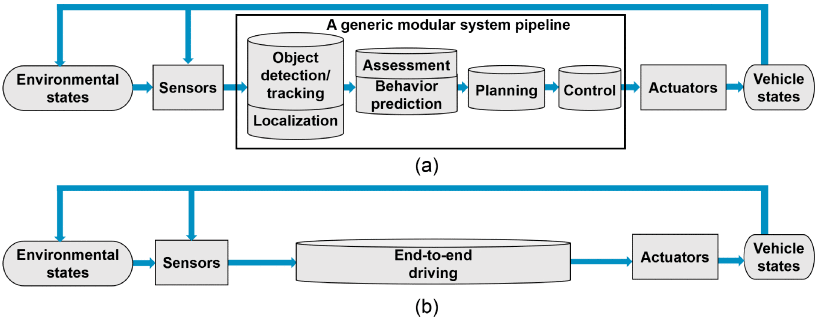
\includegraphics[width={0.9\textwidth}]{images/AD_architecture.png}
	\caption{Autonomous driving architecture: a) Modular system b) End-to-end system \cite{ad_pipeline}}
	\label{fig:ad_architercture}	
\end{figure}


The crusial role in decision making is played by action-values(Q-values). For a given state of the environment each of possible actions has its own Q-value that was calculated through accumulating the possible prospected reward to be received if the action is taken. The calculations are performed according to the following formula~\cite{xue2023dvqn}:

\[
Q_\pi(s, a) = \mathbb{E}_\pi \left[ \sum_{k=0}^\infty \gamma^k R_{t+k+1} \mid S_t = s, A_t = a, \pi \right]
\]

In DQN the approximation of the action-value for every action is performed by the neural network. Then the policy performs the action which has the highest Q-value, according to \[Q^*(s, a) = \max_\pi Q_\pi(s, a)\]. 

To leverage the criticality in transfer learning there was a complex procedure performed. The base-model, trained purely on the  \texttt{Highway-Env}, was applied to perform "testdrives" in the \texttt{Merge-Env} to collect necessary data for the future applications of transfer learning. The most important data to be collected for criticality purposes was: obserations of all the completed steps through out episodes. The model is able to give the Q-net of the observation out, which represents the Q-values for each of 5 possible actions. Based on the maximum action-value among those in Q-net, as described earlier, the algorythm was making decisions about which action to perform for a given observation. However, now, the Q-net was used in a different way: there was a statistical value of variance\cite{Karino_2020,} of Q-values found for the purpose of criticality. The variance is calculated by averaging squares of deviations from the distribution mean~\cite{variance2018}:

\[
\sigma^2 = \frac{\sum (X - \mu)^2}{N}
\]

The purpose of calculating the variance is to find the deviation of values inside of a Q-net, mainly to identify if one of action-values was reasonably higher than all others. Higher variance represents that one of actions was much likely to be taken by the policy than others. The Q-net variances of all the observations recorded should have been further analysed, ...

!!!Describe the python package to find the variance and also describe the python package and the whole method how local peaks were found !!!!

Now when observations of critical states are collected, the next goal is to use them for transfer learning of the initial Highway policy. The ordinary DQN policy is trained in the way, when the desired number of training epochs the algorithm uses initial states of the system. Those are fed into the algorithm, and based on them the policy is trained. It either explores or exploits the initial state and the following states triggered by the action taken by the existing policy. Based on this experience the agent is trained to perform the decision making in favor of one action in every given state, thus maximising rewards and, by that, the driving performance. However the crusial point of initial states ampling for the training is that this is done randomly. Meaning every initial state of the system is randomly generated: the lane of the agent, positions of surrounding vehicles, its' velocities and the velocity of agent car, everything is initialised randomly in every iteration.

The theory of this bachelor paper is, instead of set of randomised states, to feed the DQN algorithm with a set of critical states of a smaller lenth and evaluate if the acceptable performance can be acheived via this method. The set of input states is generated by the DQN interrnally. This is performed by the Replay Buffer.

\subsection{Replay Buffer}

As critical states are collected, the next processing step is feeding this set into the algorithm for purposes of transfer learning. The target is to control the input of the DQN by replacing random state samples with a list of critical states. This was realised with the use of an in-built component of DQN called Replay Buffer(or Experience Replay).

The whole idea behind the principle of experience replay is grounded in neuroscience. Observing and exploring rodents, scientists suggest that the brain replays sequences of prior experience during its sleeping and awake resting phases~\cite{Foster2006}. Based on this knowledge DQN was extended by the replay buffer, where the design is following: experience, completed once will not be erased after one iteration, but on the contrary will be stored inside of the replay buffer to be reapplied later~\cite{schaul2016prioritizedexperiencereplay}. Moreover, it becomes more probable for the rare-appearing experience samples to be learned multiple times. Utilising a mix of recent and older experience stabilises the training process.

Google DeepMind's "Prioritized Experience Replay" research towards the optimisation of the usage of replay buffer in the DQN served as an inspiration for implementation within this thesis. The paper explores one possible improvement of a general replay buffer realisation, where the DQN will utilise the set of random states in a manner, where some states will be prioritized over others. The purpose of the research is brilliantly described in one sentence: "This paper addresses only the latter: making the most effective use of the replay memory for learning, assuming that its contents are outside of our control." ~\cite{schaul2016prioritizedexperiencereplay} After digging into the prioritised replay approach, the concept of overwriting the replay buffer data came to mind. Generally, the intention, that was pursued during the development of the replay buffer, is to reduce the amount of experience required for effective learning. At the same time, we will try to take a full control of the experience set and reduce it even further.

A list of observations is not enough information, which is required to create a working buffer. Additionally, actions taken under the conditions of the state, the received reward and the resultant observations are required. To obtain the following data, the pre-trained highway model was used, which is the same model that collected critical states. Before the start of transfer model training process, the experience buffer is filled with all necessary values and connected to a system to be employed by the DQN algorithm.

		
\newpage

\thispagestyle{myPageStyle}
% Chapter - 4 
\section{Experiments, Results and Discussion}\label{chap:chap_4}
		
\newpage

\thispagestyle{myPageStyle}
\clearpage

\section{Conclusion}\label{chap:chap_5}

In the present chapter, the results, accomplishments and some shortcomings of the present thesis are summarized in Section \ref{sec:subsec_5.1}. Some ideas for future research work are highlighted in Section \ref{sec:subsec_5.2}.

% New Section: 
% -----------------
\subsection{Summary}\label{sec:subsec_5.1}

This bachelor's thesis explores leveraging criticality in RL to improve TL in the field of autonomous driving. The research aimed to identify whether a transfer to a new environment can be efficiently realised through training a model on critical states of a target environment. There were four model types developed and evaluated in the \emph{Highway-Env} and \emph{Merge-Env} to assess the impact of TL, the choice of a set of critical states, and the training methodology.

In the beginning, global metrics underwent the examination. Metrics included: collision rate, average episode time and general reward. Through that, the basic knowledge about the model's overall performance level and functionality was obtained, including the ability to handle complex scenarios. The study found that those models, which were obtained through leveraging the TL approach, outperformed models, trained in a single environment, consistently. This concerns both stability and safety. The final discovery is, that the efficienty of proposed hypothesis--leveraging criticality for effective TL--was confirmed experimentally. The consistency of results in global metrics among conducted experiments confirms the idea that the use of critical states for transfer training purposes is effective.

A new approach was introduced, which consists of performing TL purely on critical states to improve the efficiency of TL. In doing so, the focus of the training model was on challenging scenarios. This approach reduced the training step number significantly, maintaining the performance on a level compatible with conventional TL.

The model \texttt{Highway-Merge Model} that was trained with traditional TL on an array of states, sampled randomly, outperformed the \texttt{Pure Merge Model} trained on the \emph{Merge-Env} from scratch. The latter, in turn, demonstrates a higher accident rate, inconsistency of decision-making, and overall unreliability. The \texttt{Highway-Merge Criticals} model, which used a list of previously collected critical states, was showing promising results maintaining a comparable performance while diminishing training time.

Through a deep exploration of data acquired for various metrics, significant insights into the performance and behaviour of \texttt{Highway-Merge Criticals} model were obtained. Understanding the strengths and focus areas of the model was achieved through the detailed analysis of those metrics. This assisted later in the evaluation of the effectiveness.

\texttt{Highway-Merge Criticals} model was able to achieve such performance results by making behaviour adjustments. Unlike the second TL model, the target model decreased the average driving speed(based on Section~\ref{sec:overall_reward_types}) to achieve better results in accident rate and merging speed reward. This capability of criticality TL models to re-evaluate the importance of different types of rewards can further be explored.

After the analysis of results, it is clear that \texttt{Highway-Merge Criticals} model can successfully navigate merging scenarios, being trained on a noticeably smaller set of input states. At the same time, overall results depict minor fluctuations, where the future optimisation of this approach can take place.

% New Section: 
% -----------------
\subsection{Future prospects}\label{sec:subsec_5.2}

Future research can be focused on adapting an algorithm to improve the output of TL with the use of critical states. This can include the following points:

\textbf{Exploring Different Ways of Criticality Identification:} This thesis is based on critical states that were found when observing the behaviour of variance of Q-values for possible actions(Section~\ref{sec:criticality}). Evaluate the performance that could have been obtained if using improved or completely different methods to find critical states. For instance, the threshold selection method can be used to identify critical states. This, if refined in future research, may lead to a scharp rise of the effectiveness of criticality approach in TL.

\textbf{Applying Different RL Algorithms:} DQN algorithm was used throughout the paper. However, multiple RL methods exist, besides DQN, which can achieve higher performance results. For example Soft Actor-Critic(SAC) or Proximal Policy Optimisation(PPO).

\textbf{Exploring Different Replay Buffer Setups:} During the training process the pre-filled Replay Buffer was used, where critical experiences were sampled in random batches. To ensure the sampling of all critical states while training the model, it is worth attempting the application of non-random sampling, which will ensure that each critical state is sampled at least once. Moreover, while learning, the DQN did not update the Experience Replay with newly collected samples, leaving the Buffer static. Continuous appending or gradually replacing used critical states with freshly experienced states may avoid overfitting and profit training effectiveness. This leads to the deeper idea of Dynamic Criticality Sampling.

\textbf{Exploring the Dynamic Criticality Sampling:} The additional set of critical states can also be collected while training the model. Appending the Replay Buffer with newly found critical states can further improve the robustness and performance of the model.

\textbf{Scaling to More Complex Environments:} The implementation of a novel TL method was completed in between \emph{Highway-Env} and \emph{Merge-Env}. However, to validate the approach to the level where it can be applied in real-world scenarios, further investigation is required, when applying, explored above, mechanisms in more complex scenarios in the field of autonomous driving.

This paper demonstrates the approach of leveraging criticality for TL being an effective tool to boost RL in autonomous driving. The results of a validation defined a model, trained entirely on critical states, reduces training time while maintaining good effectiveness and securing the safety of the decision-making process. These results contribute to the wider RL field and autonomous vehicles in general, offering insights to be applied in future real-world realisations.

\subsection{Outcome}\label{sec:outcome}

The leveraging of criticality applied in TL demonstrates performance comparable with standard TL while requiring fewer training steps, thus less time and computation power. However, there are still some imperfections in the results and algorithm in general that need to be improved in future research.

When utilising critical states by sampling them from Replay Buffer to improve predictions of Neural Network for Q-values, the model can reach higher levels of safety and efficiency than traditional TL. Current implementation achieved those levels while, at this moment, still being less stable than ordinary TL, this was represented by wider standard deviation values in Figure \ref{fig:rewards_all}. This work shows that the model trained using critical states chooses to sacrifice the reward for higher speed to earn higher rewards for other driving aspects, like collision avoidance, merging speed or right lane occupation. Following prioritisation of rewards in a simulated environment will be reflected in a much safer and more effective behaviour of autonomous vehicles in real-world scenarios. It extracts valuable information from critical scenarios, which is then applied pointwise to train a policy to make more "thoughtful" decisions. Further research into the application of criticality can level up the TL in future, making it more accessible and widely used in various fields of everyday life.			
\newpage

	

    % Remaining part of the thesis
	\pagenumbering{Roman} 					
	\setcounter{page}{6} 						
	
	% Glossary
	\thispagestyle{myPageStyle}
	\glssetwidest{A D A S} 					
	\setglossarystyle{alttree}												
	\cleardoublepage
		
	% Literature references
	\thispagestyle{myPageStyle}
	\printbibliography
	
	% Appendices
	\thispagestyle{myPageStyle} 
	%----------Appendices-----------------------------------------------------------
\appendix

% ---------------
% Appendix A
\section{First appendix}\label{sec:subsec_6.1}

% ---------------
% Appendix B
\section{Second appendix}\label{sec:subsec_6.2}

	\cleardoublepage

\end{document}
